\documentclass{article}
\usepackage{amsmath}
\usepackage{natbib}
\usepackage{graphicx}
\usepackage{subfig}
\usepackage{bm}
\usepackage{appendix}
\usepackage{authblk}

% Special commands 
\newcommand{\vect}[1]{\boldsymbol{\mathbf{#1}}}
\providecommand{\e}[1]{\ensuremath{\times 10^{#1}}}

\title{Domestic Trade and Inequality}
\author[1]{Farid Farrokhi}
\author[2]{David Jinkins\thanks{We thank Sina Smid for research assistance, and participants in seminars at Copenhagen Business School and Cardiff University for helpful suggestions.}}
\affil[1]{Penn State}
\affil[2]{Copenhagen Business School}
\renewcommand\Authands{ and }

\begin{document}
\maketitle

Inequality has long fascinated economists, but recently rising inequality has been a topic in public forums as well.  It is not every year that a 700-page collection of charts and academic theory on inequality is a New York Times bestseller.  In this paper, we add to this discussion by documenting some new facts about the interaction of geography with inequality, and developing a model which can rationalize what we find.  After estimating the model on American data, we will discuss the effect of changes in geography on inequality.  These changes might be a new highway, or population movement due to climate change.

Our first empirical contribution is to document facts about inequality and geography.  We assign to each American city a measure of remoteness meant to capture its distance from all other cities.  We then show that this measure correlates negatively with the skill premium, the ratio of the mean wage of the highly educated to the mean wage of the less educated.  That is, highly educated workers make less relative to less educated workers in remote cities.  On the other hand, conditional on population and other controls, the more remote a city is, the higher its share of highly educated workers, which we call the college share.  As far as we know, our paper is the first to document these facts.

Previous economic geography models on inequality have treated cities as isolated rooms.  Workers in a city can interact with each other, but there is no interaction between cities.  This literature, then, has no way to discuss the interaction of geography with inequality, since the location of a city relative to other cities is irrelevant.  In order to discuss geography, we borrow heavily from recent literature on domestic trade and the size and location of cities.

% First we show theoretically that in any equilibrium model with homothetic preferences and no cost to movement between cities, the skill premium is equal everywhere.  This result holds regardless of the production technology available in different locations.  The simple intuition is that welfare must be the same everywhere for each type of worker, and sense all workers fact the same amenities and prices in each location, the skill premium must also be the same everywhere.  However, the college share, that is the share of highly-educated workers, can differ between locations.

% After developing a model with non-homothetic preferences based on patterns from the data, we show that in the abscence of agglomeration and congestion forces, larger cities will counter-factually have lower skill premia.  The intuition for this result is that less-educated workers spend a higher share of income on housing, which is more expensive in larger cities.  Thus, in order for welfare to be equal everywhere, less-educated workers need to be compensated more relative to highly-educated workers to induce them to live in a large city.  Adding agglomeration forces which differ between high and low skill workers is enough to turn this relationship around.  The positive relationship between the skill premium and city size is then indirect evidence for the presence of strong aggomeration economies for highly educated workers. 

% We present two models, one homothetic model and one non-homothetic model.  The homothetic model has a more flexible production structure, is easier to simulate, and more more closely matches the data in a number of dimensions.  We will present this model as well as simulations to understand how forces in such a geographic model affect equilibrium outcomes, especially in terms of college share.  Of course, our homothetic model is not capable of generating different wage premia in different locations.  We have also a non-homothetic model with a less flexible production structure, and which is counterfactual to the data in some dimensions.  This model can be solved, but requires an extra outer fixed point loop.  The advantage of the non-homothetic model is that it is capable of generating varying wage premia.  We hope to amalgamate these two models before we move to fully estimate the models on American data.

How does the model work?

What is the intution?

The literature on the skill premium has found a number of patterns.  To the extent that we are able to measure the relevant quantities, all of these facts are consistent with our data.  The literature has shown convincingly that the skill premium is higher in cities with larger populations 
\citep{davis2012spatial}.  The relationship between the skill premium and city size has become stronger over time \citep{baum2013inequality, lindley2014spatial}.  In addition, larger cities have been shown to have a higher share of college-educated worker, another pattern which has strengthened over time \citep{moretti2008real, lindley2014spatial}.  Areas of denser economic activity have higher skill premiums \citep{combes2012sorting}.

These stylized facts have generated a number of theories to help understand them \citep{davis2012spatial,davis2014comparative,baum2012understanding,combes2012sorting}.  These theories abstract from costly trade, treating trade between cities as either non-existant or frictionless.\footnote{\citet{davis2012spatial} does contain an extension where trade costs are treated in the limit as they go to zero.}  The style of our modeling exercise below has more in common with recent forays of trade economists into economic geography \citep{allen2014trade,desmet2014geography}.  These theories model costly trade, and focus on the spatial location of economic activity. They have, however, only one type of labor, so they cannot analyze the interaction between geography and inequality.  In an international trade context, \citet{fujita2006globalization} study inequality with costly trade, but their model has immobile unskilled workers.


Related literature

\section{Documenting inequality and geography}

In this section, we describe our data sources, give our definitions of measures of geography and inequality, and present the empirical findings which motivate our modeling exercise.  
\subsection{Data sources}

Our empirical section is based on data from the 2000 American census public use micro-data (PUMS).  In order to be consistent with the literature, we clean the data using replication code from Baum-Snow ReStat, which is available on Nathanial Baum-Snow's website.  In this cut of the data, we eliminate all workers except for white males older than 24 and younger than 55 to abstract from any considerations of sex or race discrimination.  As it stands we are left with around 1.5 million workers distributed across the United States.

We want to compare inequality in different locations.  For our purposes, a location will be a 2000 US Census Metropolitan Statistical Area (MSA).  There are more than 300 MSAs, which are economically-integrated regions.  The borders of these regions are based on county borders.  Not all American counties are part of an MSA.  In order to think about the geography of MSA's, we need to know the precise location of each MSA in space.  We download a population weighted centroid for each MSA (and PMSA) from the Missouri census data center (http://mcdc2.missouri.edu/websas/geocorr2k.html).

\subsection{Important concepts}

Our main measure of geography is remoteness, a concept we borrow from the international trade literature.\footnote{It is a famous empirical regularity that the trade of two countries is proportional to the product of their national products divided by the physical distance between them.  This relationship is known as the naive gravity equation.  The adjective naive makes an appearance because such a gravity equation implies that trade between two countries is unaffected by what takes place in a third country.  For example, the trade between the United States and Mexico is unaffected by the rapid increase in trade between China and the United States.  Remoteness in an international trade context is the national-product-weighted sum of the distance between a country and all other countries.  Multiplying the gravity equation by a remoteness term allows third countries to influence bilateral trade relationships.}  The particular functional form we use is based on a suggestion in \citet{head2003gravity}.  Let us label each MSA with a number $i=1\dots N$.  The population of MSA $i$ is $P_i$, and the geodesic distance, i.e. the distance as the crow flies, between MSA $i$ and MSA $j$ is $d_{i,j}$.  The remoteness of MSA $i$ $R_i$ is given by:

\begin{equation}
    R_i = \frac{1}{\sum_{j\neq i} \frac{P_j}{d_{i,j}}} \nonumber
    \label{eq:rem}
\end{equation}

In words, an MSA which is close to other MSA's with high populations will have low remoteness.  We want this measure to reflect the ease with which a location can trade with other locations.  This measure does not, of course, take into account geographic features such as rivers, mountains, roads, and airports, but physical distance is still an important part of transportation cost.  

We have two measures of inequality, the skill premium and the college share.  Both are measured in a way standard in the labor literature, and are calculated in each MSA.  A worker is highly educated if he has either a college degree or an academic associate degree.  The skill premium is the mean wage of highly-educated workers in an MSA divided by the mean wage of other workers.  The college share is the fraction of highly-educated workers in an MSA.  When calculating all means, we use census population weights.

In addition to our inequality variables, we define the age ratio to be the mean age of the highly educated divided by the mean age of the less educated.  Since we know from the labor literature that wages rise dramatically with age, it will be important for us to control for differences in the age profile of the two education groups in our analysis.  Ideally, we would run our analysis using only workers of approximately the same age, but such a cut reduces the size of our data dramatically and causes measures of inequality to be unreliable in smaller MSA's.  For example, including only workers within a 15-year age window reduces our data by more than half.  While it is somewhat dependent on which specific ages we choose, we get similar results in terms of both magnitudes and statistical significance if we restrict our sample to a 15-year age window rather than including age ratio as a regressor.

Table \ref{tab:sum_stats} contains some descriptive statistics.  Figure \ref{fig:geo} shows how our measures vary across the United States. In each of these figures, blue signifies a higher quantity, and red a lower quantity.  Remoteness has an obvious geographic pattern, as does the skill premium.  Remoteness is lowest in regions radiating out from New York and Chicago.  The skill premium is higher on the East Coast and in the South than it is in the Midwest and the Pacific Northwest.  It is more difficult to see an obvious geographic pattern in college share and population, except that both are higher in New England, the Pacific Northwest, and the coast of California.

\begin{table}
    \centering
    \begin{tabular}{lll}
        \hline \hline
        Statistic & Mean & Standard Dev \\ 
        \hline
        Remoteness    & 3.6\e{-6} & 1.8\e{-6} \\
        Population    & 7.3\e{5}  & 1.2\e{6}  \\
        Skill premium & 1.7       & 0.18      \\
        College share & 0.46      & 0.22      \\
        Age ratio     & 1.03      & 0.03      \\
        \hline
        Census observations & 1.1\e{6} & \\
        MSA observations    & 309      & \\
        \hline \hline
    \end{tabular}
    \caption{Data summary statistics}
    \label{tab:sum_stats}
\end{table}

\begin{figure}[!ht]
  \centering
  \subfloat[Remoteness]{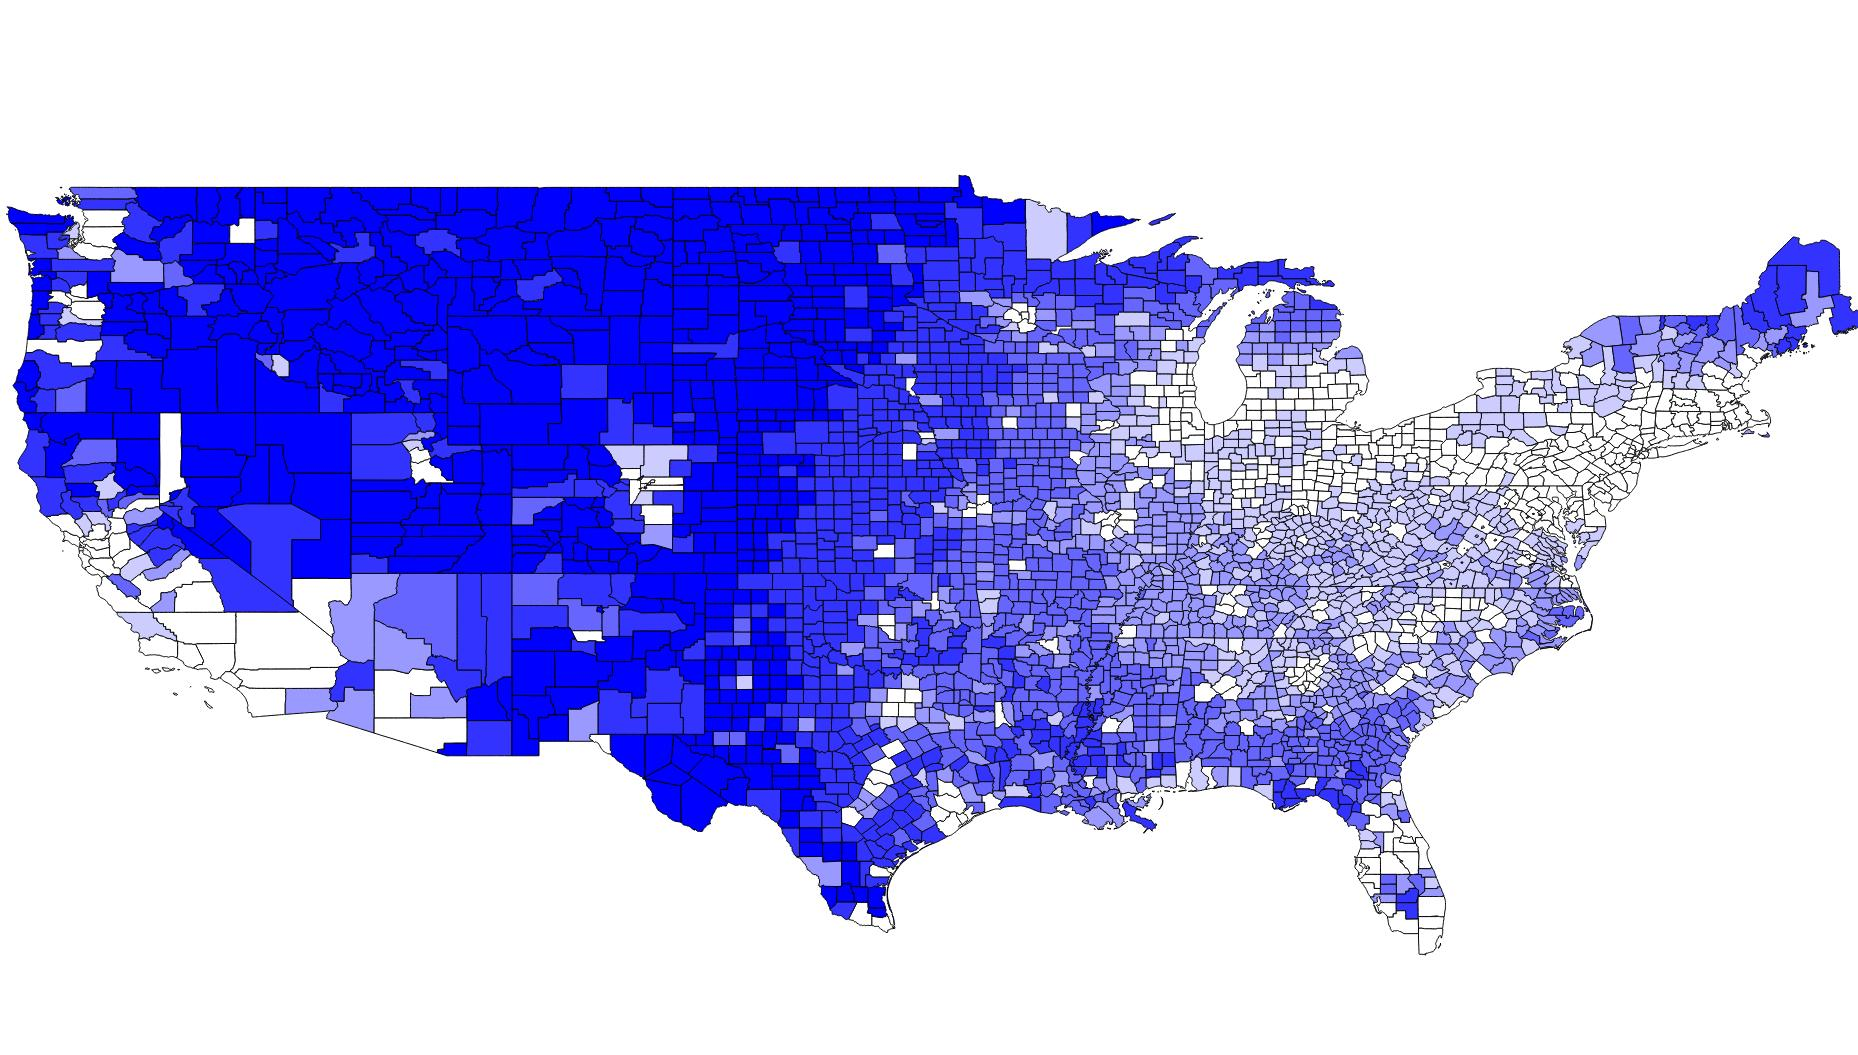
\includegraphics[width=.47\textwidth]{pics/rem.jpeg}}\quad
  \subfloat[Population]{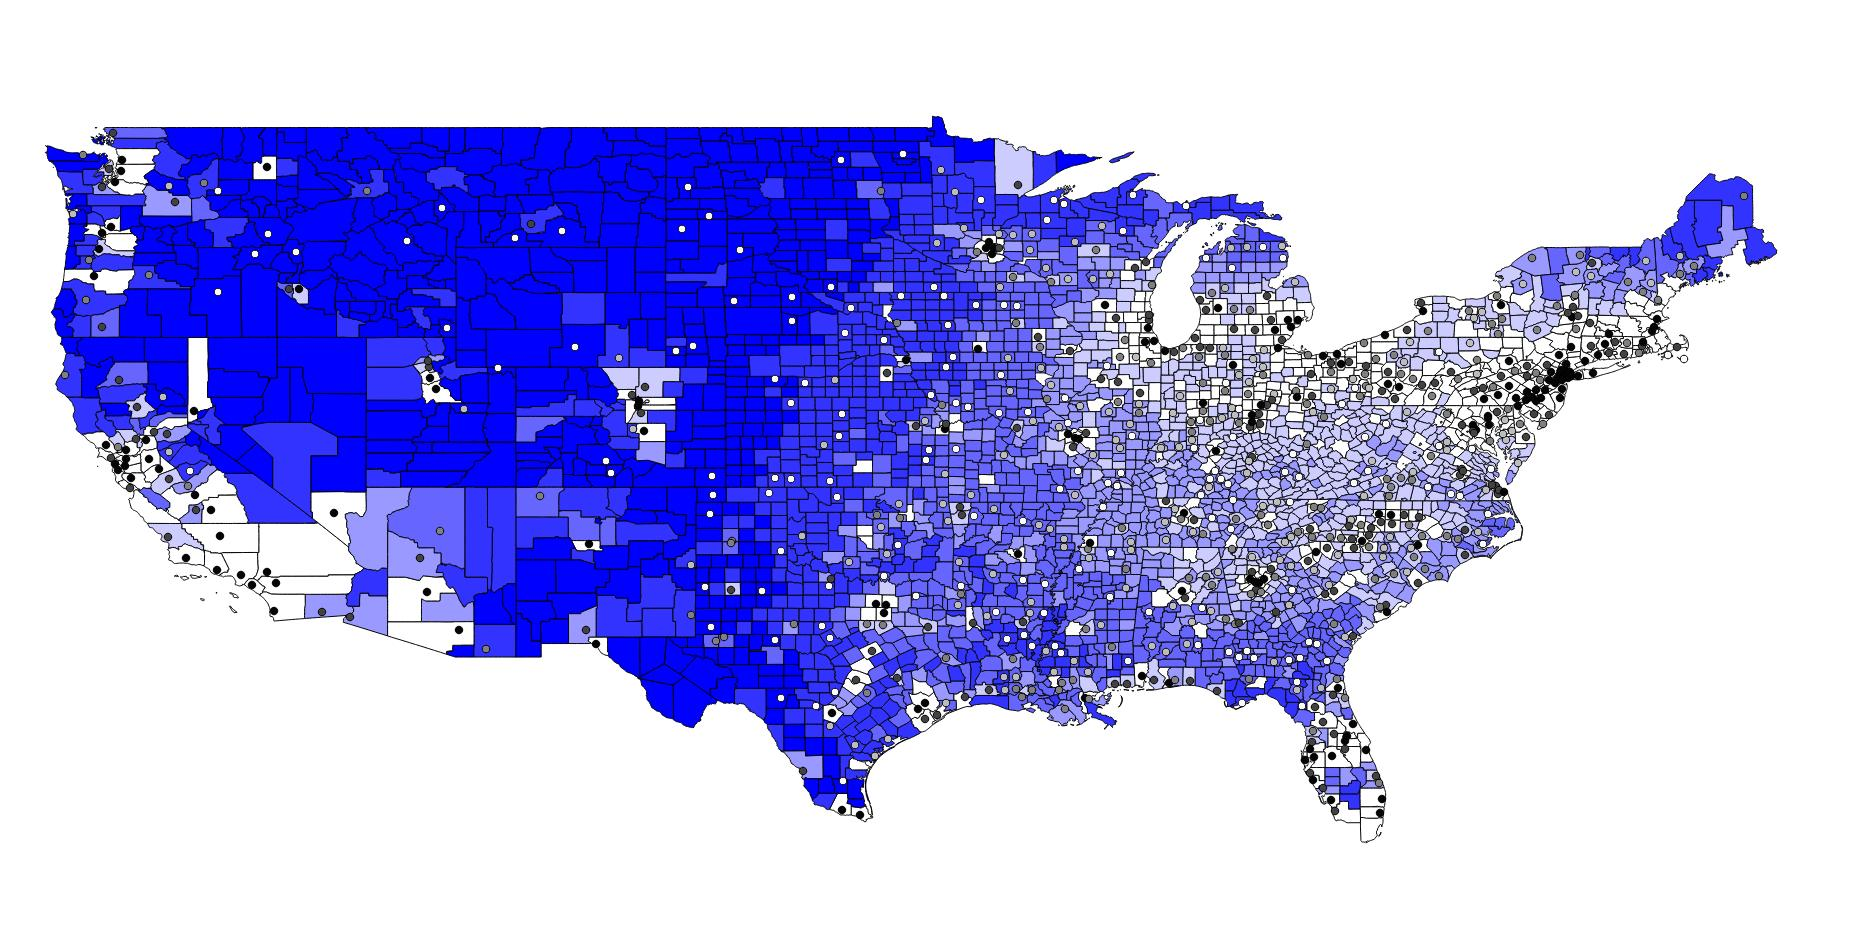
\includegraphics[width=.47\textwidth]{pics/pop.jpeg}}\\
  \subfloat[Skill Premium]{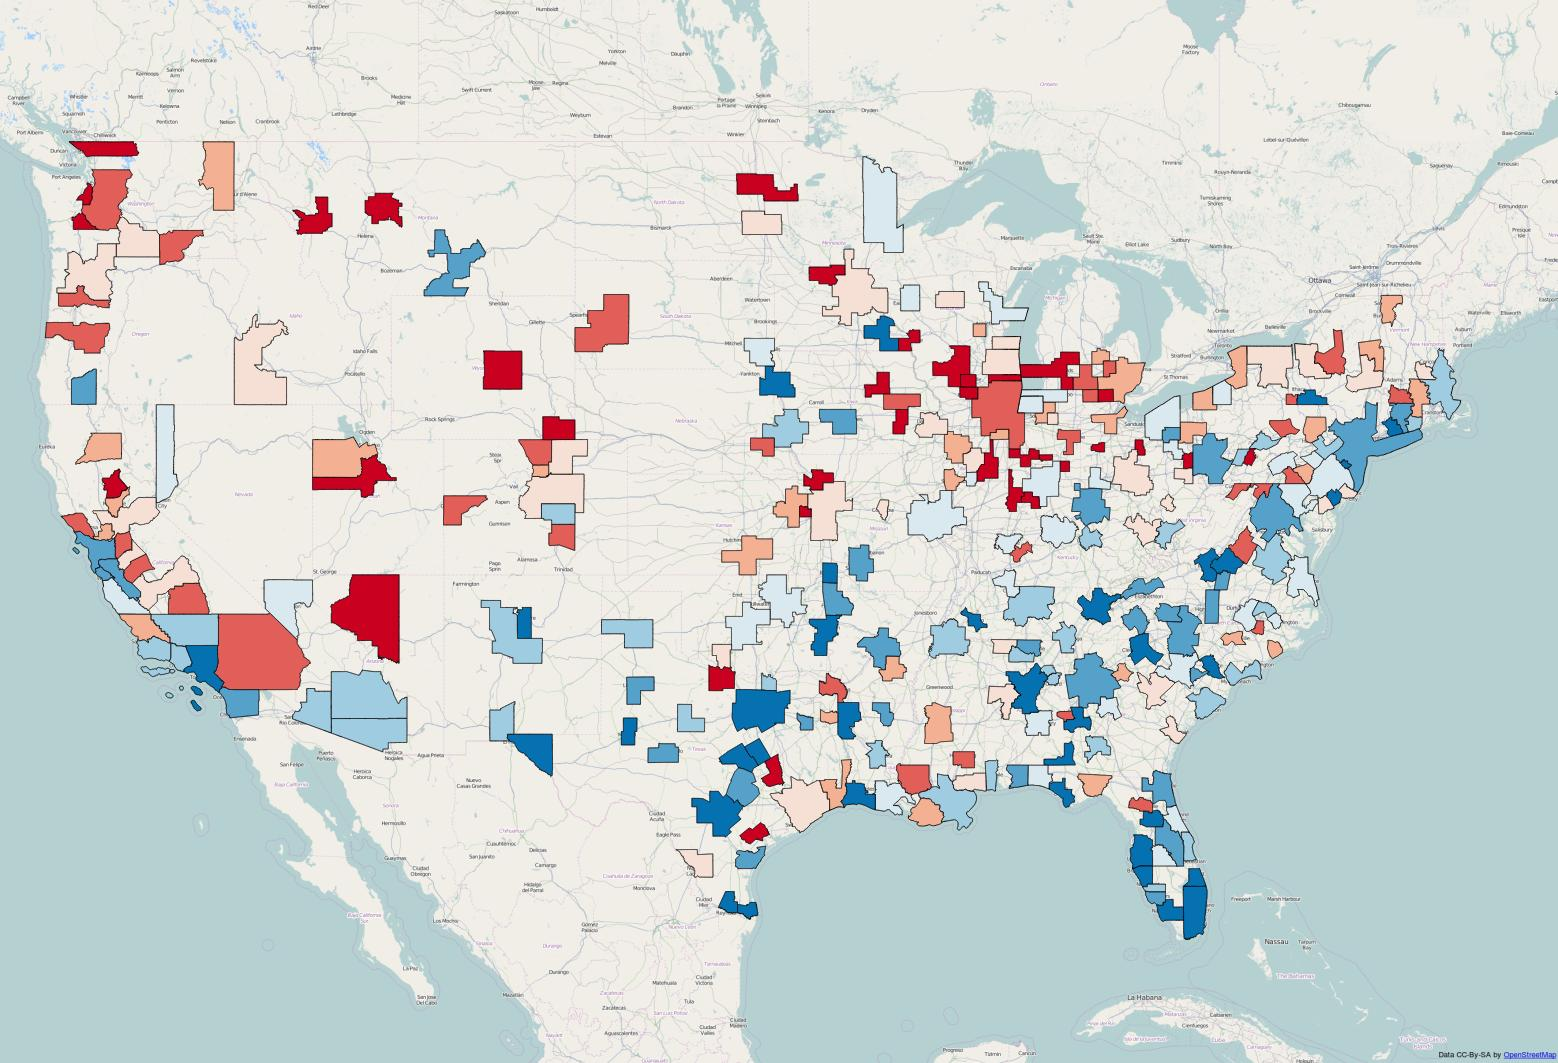
\includegraphics[width=.47\textwidth]{pics/skill_prem.jpeg}}\quad
  \subfloat[College Share]{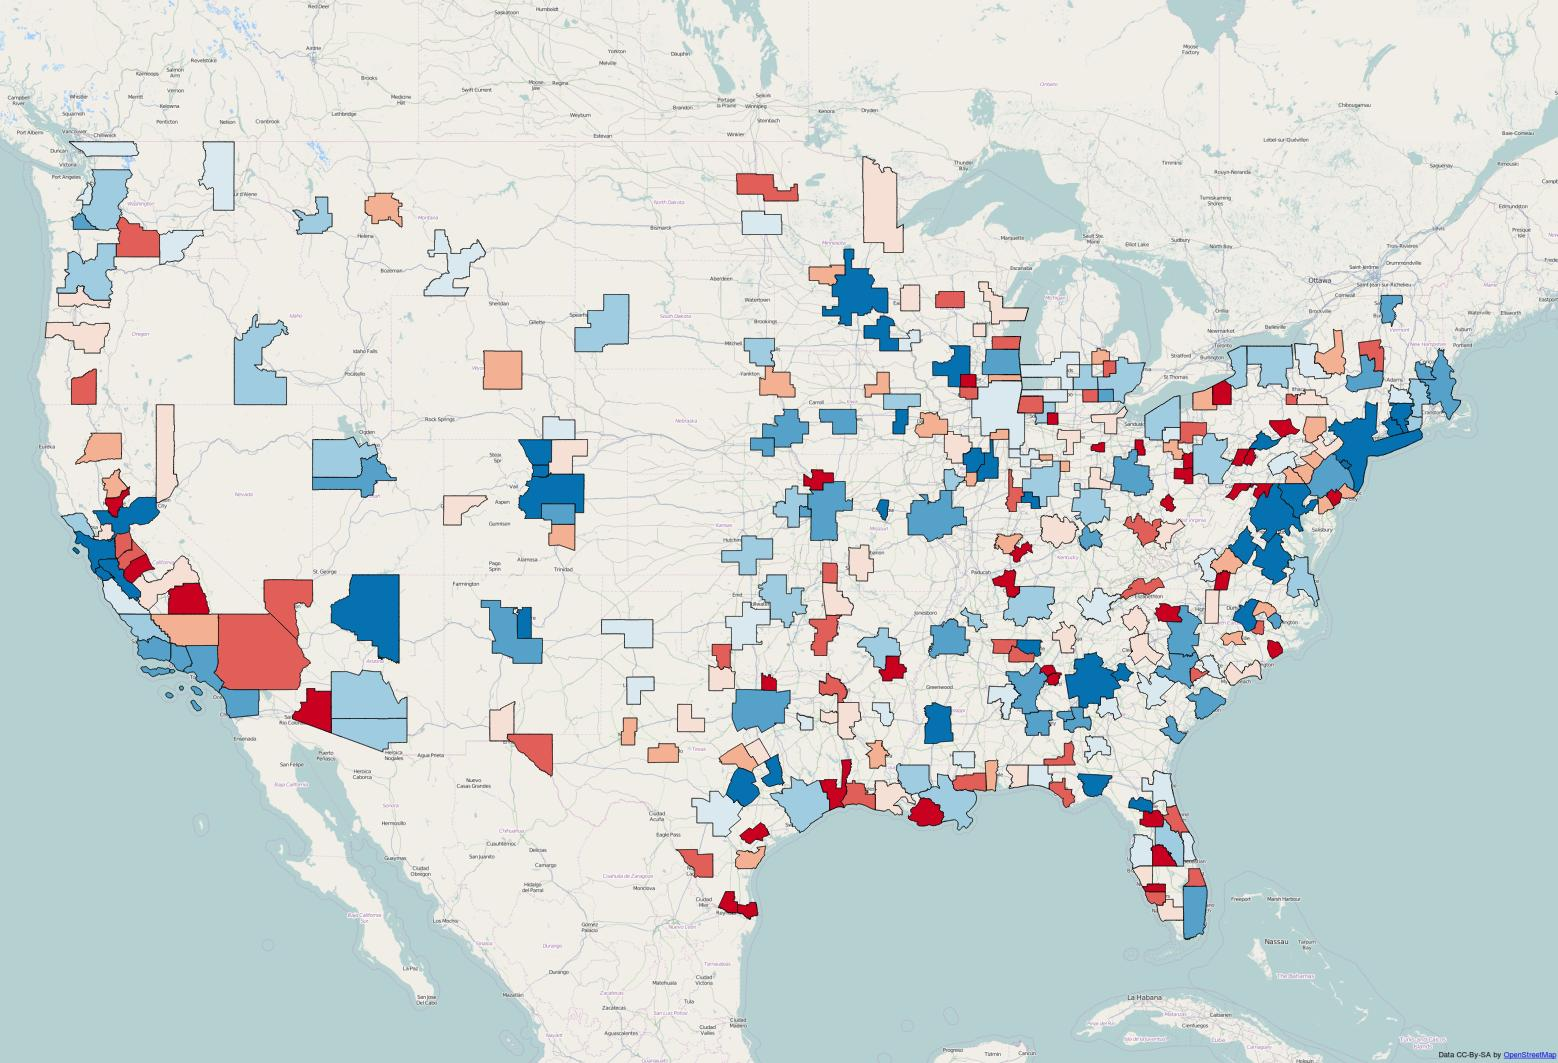
\includegraphics[width=.47\textwidth]{pics/college_ratio.jpeg}}
  \caption{MSA's by data feature}
  \label{fig:geo}
\end{figure}

\subsection{Empirical results}

% This table was done using estout package in stata, which is why the code looks so ugly!
\begin{table}
    \centering
    {
    \def\sym#1{\ifmmode^{#1}\else\(^{#1}\)\fi}
    \begin{tabular}{l*{3}{c}}
    \hline\hline
                        &\multicolumn{1}{c}{(1)}&\multicolumn{1}{c}{(2)}&\multicolumn{1}{c}{(3)}\\
                        &\multicolumn{1}{c}{Ln Skill Prm}&\multicolumn{1}{c}{Ln Skill Prm}&\multicolumn{1}{c}{Ln Skill Prm}\\
    \hline
    Ln Remote           &     -0.0133         &     -0.0452\sym{**} &     -0.0493\sym{***}\\
                        &    (0.0161)         &    (0.0180)         &    (0.0165)         \\
    [1em]
    Ln Age Rat          &                     &       0.997\sym{***}&       1.388\sym{***}\\
                        &                     &     (0.272)         &     (0.255)         \\
    [1em]
    Ln Pop              &                     &                     &      0.0411\sym{***}\\
                        &                     &                     &   (0.00535)         \\
    [1em]
    Constant            &       0.370\sym{*}  &     -0.0617         &      -0.653\sym{***}\\
                        &     (0.203)         &     (0.232)         &     (0.226)         \\
    \hline
    Observations        &         309         &         309         &         309         \\
    Adjusted \(R^{2}\)  &      -0.001         &       0.038         &       0.191         \\
    \hline\hline
    \multicolumn{4}{l}{\footnotesize Standard errors in parentheses}\\
    \multicolumn{4}{l}{\footnotesize \sym{*} \(p<0.10\), \sym{**} \(p<0.05\), \sym{***} \(p<0.01\)}\\
    \end{tabular}
    }
    \caption{Regressions of log skill premium on log geography variables}
    \label{tab:skill_reg}
\end{table}


% This table was done using estout package in stata, which is why the code looks so ugly!
\begin{table}
    \centering
    {
    \def\sym#1{\ifmmode^{#1}\else\(^{#1}\)\fi}
    \begin{tabular}{l*{3}{c}}
    \hline\hline
                        &\multicolumn{1}{c}{(1)}&\multicolumn{1}{c}{(2)}&\multicolumn{1}{c}{(3)}\\
                        &\multicolumn{1}{c}{Ln College Shr}&\multicolumn{1}{c}{Ln College Shr}&\multicolumn{1}{c}{Ln College Shr}\\
    \hline
    Ln Remote           &     -0.0209         &       0.199\sym{***}&       0.182\sym{***}\\
                        &    (0.0650)         &    (0.0696)         &    (0.0632)         \\
    [1em]
    Ln Age Rat          &                     &      -6.880\sym{***}&      -5.289\sym{***}\\
                        &                     &     (1.052)         &     (0.974)         \\
    [1em]
    Ln Pop              &                     &                     &       0.167\sym{***}\\
                        &                     &                     &    (0.0205)         \\
    [1em]
    Constant            &      -1.131         &       1.846\sym{**} &      -0.557         \\
                        &     (0.821)         &     (0.894)         &     (0.863)         \\
    \hline
    Observations        &         309         &         309         &         309         \\
    Adjusted \(R^{2}\)  &      -0.003         &       0.117         &       0.273         \\
    \hline\hline
    \multicolumn{4}{l}{\footnotesize Standard errors in parentheses}\\
    \multicolumn{4}{l}{\footnotesize \sym{*} \(p<0.10\), \sym{**} \(p<0.05\), \sym{***} \(p<0.01\)}\\
    \end{tabular}
    }
    \caption{Regressions of log college share on log geography variables}
    \label{tab:col_reg}
\end{table}

In this section we document the covariance of our measure of geography, remoteness, with our measures of inequality, the skill premium and college share.  Regressions of the skill premium on remoteness and other variables are found in Table \ref{tab:skill_reg}.  Remoteness covaries negatively with the skill premium, although the coefficient is not significant untless the age ratio is included in the regression.  We find that the population of an MSA varies positively with the skill premium, a result that has been emphasized in other studies.  The covariance of remoteness and the skill premium is nearly the same size as its covariance with population, but in the opposite direction.

In Table \ref{tab:col_reg} we report coefficient estimates from regressions of college ratio on the same regressors.  We find that remoteness covaries positively with the college premium, and as before the effect is only significant after controling for the age ratio.  This effect is surprising, as one might expect highly-educated workers to be disproportionately drawn to large cities in areas with low remoteness.  On the other hand, it makes sense that in remote areas where the skill premium is lower, we should find a larger relative supply of highly-educated workers.  As before, the magnitude of the population effect and the remoteness effect are similar.

We have strong intuition for why the age ratio is positively correlated with the skill premium.  Older people earn more, so if highly-educated workers are older than less-educated workers, the skill premium will be higher.  We do not have such strong intuition for the strong negative correlation between the college share and the age ratio.  In words, MSA's with a high fraction of highly-educated workers, have relatively young highly-educated workers.

An alternative method of controling for the age of workers is to limit our analysis to workers in a smaller age range.  Doing this significantly reduces the data available for us to calculate our regressors accurately.  As a robustness check, we present results in the appendix for only workers 35 to 50 years old.  The results are nearly the same as those found in our main analysis.

\section{Theory}

In the last section, we presented evidence that geography plays a role in shaping the skill premium and college shares.  In this section we develop models to help us understand the patterns we found, in particular that the skill premium decreases with the remoteness of a location, while the college share increases.  First we show that if preferences are homothetic, in any spatial equilibrium model there will be no difference in the skill premium between locations.  We then show how a model with non-homothetic preferences is able to deliver varying skill premia.  Finally we discuss how such a model might be estimated.

\subsection{No Skill Premia Variation with Homothetic Preferences}

Workers have homothetic preferences of the form:

\begin{equation}
    U(\bm{c}) = u(\bm{c}) a \nonumber
    \label{eq:homo}
\end{equation}

Subject to:

\begin{equation}
    w = \bm{p} \bm{c}  \nonumber
    \label{eq:homobc}
\end{equation}

In the above preferences, $a$ is amenities, $\bm{c}$ is a vector of consumption, $\bm{p}$ is a vector of prices, and $w$ is the wage.  Because preferences are homothetic, indirect utility can be written: 

\begin{equation}
    U(\bm{p},w) = w f(\bm{p}) a \nonumber
    \label{eq:homoin}
\end{equation}

The form of $f$ depends on the specific functional form of $u$.  Now suppose we have two locations, $1$ and $2$, and two types of workers $h$ and $l$.  Amenities, wages, and prices are all different in the two locations, and wages differ across types as well.  In a spatial equilibrium model with free movement between locations, welfare in any populated location must be equalized within a type.

\begin{align}
    w_{h,1} f(\bm{p}_{1}) a_{1} &= w_{h,2} f(\bm{p}_{2}) a_{2} \nonumber \\
    w_{l,1} f(\bm{p}_{1}) a_{1} &= w_{l,2} f(\bm{p}_{2}) a_{2} \nonumber
\end{align}

Divinging the two welfare equalization conditions, we see that the skill premium will be the same in any location populated with both type of worker.

\begin{equation}
    \frac{w_{h,1}}{w_{l,1}} = \frac{w_{h,2}}{w_{l,2}} \nonumber
\end{equation}

The equalization of the skill premium does not depend on the production structure of the economy, or the geography between cities.  It also does not require that the share of types be the same in any two locations.

\subsection{Non-homothetic preferences}

We have shown that we need to use a non-homothetic utility function in our model if we want to capture the dependence of the skill premium on geography.  There are, of course, many different ways for preferences to be non-homothetic.  To guide our modeling, we examine household expenditure on housing.   Housing is a large share of household expenditure, and research on the welfare effects of trade barriers has focused on the housing stock, or at least some non-tradable consumption good in fixed supply \citep{helpman1998size,redding2008costs}.  We examine how the share of a household's expenditure on housing varies with income.  This relationship is sometimes called an Engel curve.

\begin{figure}
    \begin{center}
        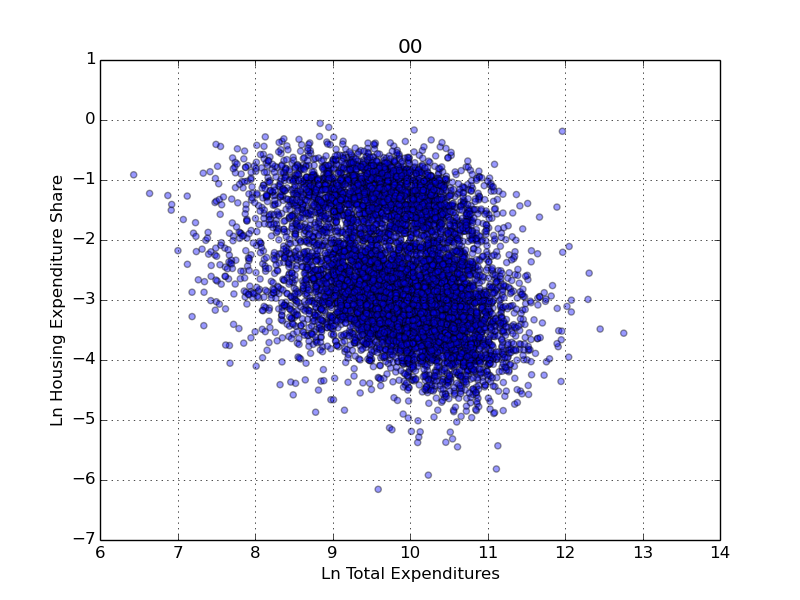
\includegraphics[width=4in]{pics/rent_shr_wage_scatter_00.png}
    \end{center}
    \caption{2000 American imputed annual rent over total expenditures}
    \label{fig:wage_rent}
\end{figure}

If preferences were homothetic, we would expect income to be unrelated to the share of total expenditure spent on housing.  Figure \ref{fig:wage_rent} contains share of spending on housing over total spending created from the American Consumer Expenditure Survey.  The measure of housing spending is actual rent if available, and imputed rent for homeowners.  We see that as expenditure increases, the share of expenditure spent on housing decreases.  We use total expenditure rather than total income because the rich save more than the poor, so that spending as a share of income is decreasing in every category of spending.

\subsubsection{Preferences and production technology}

In order to capture the decreasing Engel curve, we use Stone-Geary preferences.  A worker needs to consume a certain amount of housing $k_0$ before he can enjoy any other consumption.  As above, there are two types of labor, high-skilled $H$ and low-skilled $L$, and it is convenient for us to assume that high-skill labor produces a tradeable good, while low-skill labor produces a local non-tradable.  A final consumer with budget $y$ in location $i$ maximizes welfare,

\begin{eqnarray}
	\max \limits_{q_H(s,i),~q_L(i),~z} ~
	\left(\left[\int_S q_H(s,i)^{\frac{\sigma - 1}{\sigma}}~ ds\right]^{\frac{\sigma}{\sigma-1}}\right)^{\gamma_H} q_L(i)^{\gamma_L} (z-z_0)^{1-\gamma_H-\gamma_L} \nonumber
\end{eqnarray} 
subject to
\begin{eqnarray}
	y = p_z(i) z + p_L(i)q_L(i) + \int_S p_H(s,i)q_H(s,i) ds  \nonumber
\end{eqnarray}

Here, $H$ and $L$ index goods produced by high- and low-skilled labor. $H$ is differentiated by location of production and is tradable, while $L$ is a nontradable bundle to be locally produced. $z$ is the consumption of local housing.  We currently do not have amenities here, but they would be straight-forward to add.

Labor is the only factor of production, and define $A_H(i)$ to be the units a high-skilled worker produces in one hour.  We will call this the productivity of high-skilled labor in location $i$.  Let $w_H(i)$ the wage of high-skilled labor in location $i$, and $d(s,i) \geq 1$ be the iceberg trade costs of shipping an high-skill good from $s$ to $i$.  That is, in order to have one unit of the good arrive in $i$, a producer in $s$ needs to ship $d(s,i)$ units of the good.  We that markets are perfectly competitive, so that the price $p_H(s,i)$ of the good produced in $s$ and sold in location $i$ is $w_H(s)d(s,i)/A_H(s)$ Similarly define $A_L(i)$, $w_L(i)$, and $p_L(i)$. 

\subsubsection{Optimal consumer expenditure}

Given wages and productivities, optimal expenditures of a consumer in location $i$ with income $y$ are given as follows:
\begin{eqnarray}
	X_H(s,i;y) & = & \Big[ \frac{p_H(s,i)}{P_H(i)} \Big]^{1-\sigma} \gamma_H (y-p_z(i)z_0) \nonumber \\
	X_L(i;y)   & = & \gamma_L (y-p_z(i)z_0) \nonumber \\
	X_z(i;y)   & = & (1-\gamma_H-\gamma_L)(y-p_z(i) z_0)+p_z(i)z_0 \\
    \label{eq:house_demand}
\end{eqnarray}
where the price index of the differentiated good is
\begin{eqnarray}
    \label{eq:nonhomo_price_index}
	P_H(i) = \left[\int_S p_H(s,i)^{1-\sigma}~ ds\right]^{\frac{1}{1-\sigma}}
\end{eqnarray} 
We can now verify that the share of spending on housing is decreasing in income, and equal to $(1-\gamma_H-\gamma_L)+(\gamma_H+\gamma_L){p_z(i)z_0}/{y}$. 
Indirect utility of a worker in location $i$ with income is $y$ is
\begin{eqnarray}
	W(i;y)  =  \frac{y-p_z(i)z_0}{P(i)} \nonumber
\end{eqnarray}
where the ideal price index is
\[
	P(i)  = \gamma_{0}
	P_H(i)^{\gamma_H}p_L(i)^{\gamma_L}p_z(i)^{1-\gamma_H-\gamma_L},
\]
with $\gamma_{0}=\gamma_H^{-\gamma_H} \gamma_L^{-\gamma_L}(1-\gamma_H-\gamma_L)^{-(1-\gamma_H-\gamma_L)}$.

\subsubsection{Equilibrium Conditions}

As is standard in the economic geography literature, we assume that workers are freely mobile between locations.  This implies that within each type welfare must be the same in any location.  Replace $y$ with $w_H(i)$ for high-skilled labor and $w_L(i)$ for low-skilled labor.  Welfare equalization implies that for all populated locations $i$, we have
\begin{eqnarray}
	W_L = \frac{w_L(i)-p_z(i)z_0}{P(i)} , ~ 	
	W_H = \frac{w_H(i)-p_z(i)z_0}{P(i)}
    \label{eq:weleq}
\end{eqnarray}

Next we have the market clearing conditions.  Let $N(i)$, $N_H(i)$ and $N_L(i)$ be measures of total, high- and low-skilled labor in location $i$.  $X_H(s,i)$, $X_L(i)$, $X_z(i)$ be aggregate spending in each location.  The supply of housing in each location is the same and equals $\bar{Z}$. Market clearing conditions for high-skilled labor, low-skilled labor, and housing are given by
\begin{eqnarray}
	(mcc_H) & & w_H(i) N_H(i) = \int_S X_H(i,s) ds  \nonumber \\
	(mcc_L) & & w_L(i) N_L(i) = X_L(i) \nonumber \\
	(mcc_z) & & p_z(i) \bar{Z} = X_z(i)  \nonumber
\end{eqnarray}

We have to take a stand on who receives the payments for local endowments. In each location $i$, there is a measure one of housing owners whose total income is $p_z(i) \bar{Z}$.  These capitalists do not participate in labor market, and only consuming what they earn by housing renting their housing to perfectly competitive housing firms.  Total population in $i$ is then $N(i)=N_H(i)+N_L(i)+1$, and total income, denoted by $Y(i)$, is given by
\[
	Y(i) = w_H(i) N_H(i) + w_L(i) N_L(i) + p_z(i) \bar{Z}
\]

Define a distribution of economic activity to be a set of $w_H$, $w_L$, $N_H$, and $N_L$ with normalization $\int_S w_H(s)~ ds =1$. A distribution of economic activity is a spatial equilibrium if welfare is equalized across populated locations, goods markets clear in each location, and the sum of populations local populations is equal to exogenously given aggregates, $\int_S N_L(s) ~ds = \bar{N}_L$ and $\int_S N_H(s) ~ds = \bar{N}_H$.

\subsubsection{Solving the model}

We can reduce the model to two equilibrium conditions reminescent of those derived in \citet{allen2014trade}.  This is important, because having the equilibrium conditions in a similar form will allow us to use both the same existence and uniqueness results as that paper and also an iterative procedure for finding the equilibrium.\footnote{We won't be able to get a clean parameter condition for existance and uniqueness as in \citet{allen2014trade}, but we can numerically show uniqueness for a set of parameters.  Also, our estimation algorithm will have to be somewhat more involved.  More on both points later.}

Our first equilibrium condition is:

\begin{eqnarray}
	& & N_H(i) w_H(i)^{\sigma}   = \nonumber \\
	& & \int_S W_H^{1-\sigma} m(s)^{1-\sigma} d(i,s)^{1-\sigma} A_H(i)^{\sigma-1} g(s)^{\sigma-1} N_H(s) w_H(s)^{\sigma}~ds  \nonumber
    \label{eq:equib1}
\end{eqnarray}

And our second is:

\begin{eqnarray}
 	w_H(i)^{1-\sigma} = \int_S W_H^{1-\sigma} m(i)^{1-\sigma} d(s,i)^{1-\sigma} A_H(s)^{\sigma-1} c(i)^{\sigma-1}  	w_H(s)^{1-\sigma} \nonumber
 	~ ds
    \label{eq:equib2}
\end{eqnarray}

The only difference between our conditions, and those in \citet{allen2014trade} are the presence of the functions $m$ and $g$.  These are given below:

\begin{eqnarray}
    \label{eq:end1}
	m(i)  & \equiv & \frac{P(i)}{P_H(i)} \\
    \label{eq:end2}
	g(s) & \equiv & 1- \frac{(1-\gamma_H -\gamma_L)N_H(s)z_0}{\gamma_H (\bar{Z}-N(s)z_0)}
\end{eqnarray}

These additions are not trivial, as they involve endogenous objects -- prices in the case of \eqref{eq:end1} and populations in the case of \eqref{eq:end2}.  Prices $P(i)$ and $P_H(i)$ and total populations $N(i)$ appear nowhere else in the equilibrium conditions.  We have yet to simulate this model, but to solve for equilibrium will conceptually involve a traditional iteration on a fixed point -- taking $c$ and $m$ as given, solve the model, and then use the model's solution to update $c$ and $m$ and resolve, etc.

\subsubsection{Discussion}

We have developed an empirical model of geography and non-homothetic preferences.  Before taking it to the data, however, we can learn something from simply examining the relationships in the model.  One key empirical feature we want to match is the relationship between remoteness/population and the skill premium.  From \eqref{eq:weleq}, we get the following:

\begin{equation}
	\frac{W_H}{W_L} = \frac{w_H(i)-p_z(i)z_0}{w_L(i)-p_z(i)z_0}
    \label{eq:exam_prem}
\end{equation}

A side note here is that we have also tried a totally different set of non-homothetic preferences similar to those in \citet{fajgelbaum2011income}, and in that version we get a very similar relationship.  Consider raising wages for low and high skill workers proportionally.  This will cause the right-hand side of \eqref{eq:exam_prem} to decrease.  Since we expect agglomeration to raise nominal wages in larger, less remote cities, this force makes the wage premium covary positively with population.  On the other hand, suppose that we raise the price of housing.  This causes the right-hand side of \eqref{eq:exam_prem} to increase, which pushes the wage premium to be lower in cities with higher housing prices.  Since we expect larger and less remote cities to have higher housing prices, this force makes the wage premium vary negatively with population.  Since we know the skill premium is higher in larger cities, loosely, we expect agglomeration to dominate congestion.

There are several drawbacks to this non-homothetic model.  The most important is the presence of endogenous variables in the equilibrium condition, which complicates numerical solution.  While this is unfortunate, it seems that this will likely be the case in any non-homothetic version of the model, which is necessary to drive differences in wage premia across cities.  A second drawback is the asymmetry and rigidity of the production function.  High skill workers make tradables, while low skill workers make goods that cannot be traded at all.  The factors are specific to their own good, and cannot be substituted.  In the next section, we present an empirical homothetic model which will not contain any endogenous variables in the equilibrium condition, and will have a more natural production function combining substitutable high and low-skill goods into a single final consumption good. 

\subsection{Homothetic preferences with CES production}

In this section we present a empirical model with homothetic preferences, but which has several attractive features.  First of all, the model will be easily estimable.  We have already written code to simulate the model, and we will present some lessons we have already learned from calibration.  A second attractive feature is a production function which allows for substitution between high and low-skill labor in the production of a single final consumption good.

\subsubsection{Preferences and production technology}
A final consumer of type $\tau$ in location $i$ maximizes welfare,
\begin{eqnarray}
	\max \limits_{q_{\tau}(s,i)} ~
	\left[\int_S q_{\tau}(s,i)^{\frac{\sigma - 1}{\sigma}}~ ds\right]^{\frac{\sigma}{\sigma-1}} u(i) \nonumber
\end{eqnarray} 
subject to
\begin{eqnarray}
	w_{\tau} = \int_S p(s,i)q_\tau(s,i) ds  \nonumber
\end{eqnarray}
Goods are differentiated by the origin of production. $q_{\tau}(s,i)$ is consumer $\tau$'s consumption in $i$ from goods originated in location $s$. As we will simulate this model, we include amenities as well, which we abstracted from in the non-homothetic model above.  $u(i)$ is the utility from amenities in location $i$.

There are two types of individuals, $\tau \in \{H,L\}$ as high- and low-skilled labor. Production in each location is modeled as a CES combination of high- and low-skilled inputs
\begin{eqnarray}
	 A(i)\Big[ \beta_H(i) N_H(i)^{\frac{\varepsilon-1}{\varepsilon}} + \beta_L(i) N_L(i)^{\frac{\varepsilon-1}{\varepsilon}} \Big]^{\frac{\varepsilon}{\varepsilon-1}} \nonumber
\end{eqnarray}
where $A(i)$, $N_H(i)$, and $N_L(i)$ are respectively the total factor productivity, measure of high-skilled, and measure of low-skilled labors in location $i$. $\varepsilon>0$ is the elasticity of substitution between high and low skilled labor. $\beta_H(i)>0$ and $\beta_L(i)>0$ are factor intensities. Differences in factor intensities are the primary source of labor heterogenity in the model.  

By cost minimization, the unit cost of production equals
\begin{eqnarray}
    \label{eq:homo_cost_min}
	 \frac{c(i)}{A(i)} ,~where~~c(i)=\Big[ \beta_H(i)^{\varepsilon} w_H(i)^{1-\varepsilon} + \beta_L(i)^{\varepsilon} w_L(i)^{1-\varepsilon}\Big]^{\frac{1}{1-\varepsilon}}
\end{eqnarray}
where $w_H(i)$ and $w_L(i)$ are wages of high-skilled and wage of low-skilled labor in location $i$. 
Share of spending of producers on high-skilled labor, denoted by $b(i)$, is given by
\begin{eqnarray}
    \label{eq:def_b}
	b(i) = \frac{\beta_H(i)^{\varepsilon} w_H(i)^{1-\varepsilon}}{\beta_H(i)^{\varepsilon} w_H(i)^{1-\varepsilon} + \beta_L(i)^{\varepsilon} w_L(i)^{1-\varepsilon}}
\end{eqnarray}

Because we want to simulate the model, we need to be explicit about agglomeration.  We  assume that $\beta_H(i)=\bar{\beta}_H N_H(i)^{\alpha_H}$ and $\beta_L(i) = \bar{\beta}_L N_L(i)^{\alpha_L}$.  Agglomeration in a location for a particualr type of worker only depends on the number of workers of the same type.

\subsubsection{Market Structure, Trade, Indirect Utility.}

Let $d(s,i)$ be the trade costs of shipping a good from $s$ to $i$. With perfectly competitive markets, price of a good produced in location $s$ and consumed in location $i$, $p(s,i)$, equals $c(s)d(s,i)/A(s)$. An individual of type $\tau$ in location $i$ spends $x_\tau(s,i)$ on goods produced in $s$,
\begin{eqnarray}
    \label{eq:homo_demand}
	x_\tau(s,i) & \equiv & p(s,i) q_\tau(s,i) = \Big[ \frac{p(s,i)}{P(i)} \Big]^{1-\sigma} w_\tau(i) 
\end{eqnarray}
where 
\begin{eqnarray}
    \label{eq:homo_price_index}
	P(i) = \left[\int_S p(s,i)^{1-\sigma}~ ds\right]^{\frac{1}{1-\sigma}} \nonumber
\end{eqnarray}
Indirect utility of the consumer in location $i$ with income $w_\tau(i)$ is given by
\begin{eqnarray}
	W_\tau(i) & = & \frac{w_\tau(i)}{P(i)}u(i). \nonumber
\end{eqnarray}

\subsubsection{Equilibrium Conditions}
Let $X(s,i)= N_H(i)x_h(s,i) + N_L(i)x_l(s,i)$.  The goods market clearing condition is summarized by
\begin{eqnarray}
    \label{eq:homo_mcc}
	w_H(i) N_H(i) =  b(i) \int_S X(i,s) ds 
\end{eqnarray}
Welfare equalization is give by
\begin{eqnarray}
	W_L = \frac{w_L(i)}{P(i)}u(i) , ~ 	 \nonumber
    \label{eq:homo_wel_eq}
	W_H = \frac{w_H(i)}{P(i)}u(i) 
\end{eqnarray}

As before, a distribution of economic activity is a set of $w_H$, $w_L$, $N_H$, and $N_L$. A spatial equilibrium is a distribution of economic activity such that welfare is equalized and $\int_S N_H(s) ~ds = \bar{N}_h$ and $\int_S N_L(s) ~ds = \bar{N}_L$.

\subsubsection{Solving the model}

The full derivation is in the appendix.  As in the non-homothetic case, through manipulating and reducing the market clearing and welfare equilization conditions, we can reduce the equilibrium conditions to the following two conditions:

\begin{eqnarray}
    \label{eq:homo_eq_1}
	& & w_H(i)^{\sigma} N_H(i) b(i)^{-1} \nonumber \\
	& & =  
	W_H^{1-\sigma} A(i)^{\sigma-1} \tilde{c}(i)^{1-\sigma}
	\int_S d(i,s)^{1-\sigma} u(s)^{\sigma-1} w_H(s)^{\sigma} N_H(s) b(s)^{-1}  ~ds \\
    \label{eq:homo_eq_2}
 	& & w_H(i)^{1-\sigma} =  W_H^{1-\sigma} u(i)^{\sigma-1} 
 	\int_S  d(s,i)^{1-\sigma} A(s)^{\sigma-1}  \tilde{c}(s)^{1-\sigma} w_H(s)^{1-\sigma}
 	~ ds
\end{eqnarray}

Equations \eqref{eq:homo_eq_1} and \eqref{eq:homo_eq_2} give us two systems of integral equations. By the following relation, we can reduce the two systems into one: 
\begin{eqnarray}
    \label{eq:homo_alt_eq}
	\frac{w_H(i)^{\sigma}N_H(i)A(i)^{1-\sigma}\tilde{c}(i)^{\sigma-1}}{b(i)} = \phi w_H(i)^{1-\sigma} u(i)^{1-\sigma}
\end{eqnarray}
where $\phi > 0$ is a constant. As long as \eqref{eq:homo_alt_eq} holds, then system \eqref{eq:homo_eq_1} holds if and only if system \eqref{eq:homo_eq_2} holds. Any solution to two of the three systems \eqref{eq:homo_eq_1} - \eqref{eq:homo_alt_eq} is an equilibrium.

\subsubsection{Discussion}

As this version of the model is homothetic, it does not deliver varying skill premiums across locations.  There is a single skill premium everywhere.  On the other hand, college shares can vary.  Consider the \eqref{eq:homo_col_share} in the appendix, which is implied by the equilibrium conditions of the homothetic model.  For convenience, the relation is reproduced here:

\begin{eqnarray}
	\frac{W_H}{W_L} = \frac{\bar{\beta}_H}{\bar{\beta}_L} \frac{N_H(i)^{\tilde{\alpha}_H /\varepsilon}}{N_L(i)^{\tilde{\alpha}_L/\varepsilon}} \nonumber
\end{eqnarray}
where $\tilde{\alpha}_\tau \in [-1,\infty]$ are parameters reflecting the strength of agglomeration forces.  Generically a proportional increase in the high and low-skill populations will violate this relationship, so city size will have an influence on college share.  Exactly how geography and city size interact with college share will be discussed in the following section.

\section{Simulation of Homothetic model}

The intuition for algorithm for solving the homothetic model is to guess high skill populations $N_H(i)$, then use equilibrium relationships to calculate the rest of the distribution of economic activity.  Next use \eqref{eq:homo_eq_2} to update the original $N_H(i)$ and iterate until there is no change in $N_H(i)$.  The full algorithm is described in the appendix.

For the simulation, we consider a simple geography: three cities on a line.  Iceberg trade costs for moving one step along the line are given by $tc$.  The middle city is less remote than the two edge cities.  This model has many parameters for us to manipulate.  The somewhat arbitrary baseline paramter values are given in the Table \ref{tab:baseline}.  The baseline parameters are only somewhat arbitrary, because they reflect the findings and conventions of the literature.  Agglomeration forces are stronger for high-skill workers than for low-skill workers.  The elasticity of substitutions are both greater than one, so that goods are substitutes in utility and workers are substitutes in production.  $\beta$ is closely tied to the skill premium, and is set greater than $0.5$ so that the premium is positive.  Trade costs are such that an exporter shipping to an adjacent city needs to send 1.5 units of a good if he wants 1 unit to arrive.  This is in line with what has been found in the domestic trade cost literature (cite Tombe and Donaldson).

    \begin{table}
        \centering
        \begin{tabular}{lll}
           \hline \hline
           Parameter    & Baseline Value & Description                                     \\ \hline
           $tc$         & 0.5            & one step trade cost                             \\
           $\sigma$     & 3              & elas. of sub. across goods                      \\
           $\epsilon$   & 1.1            & elas. of sub. across labor                      \\
           $\gamma_U$   & 0.1            & congestion strength                             \\
           $\beta_H$    & 0.55           & high factor intensity ($\beta_L = 1 - \beta_H$) \\
           $\alpha_H$   & 0.02           & high agglomeration strength                     \\
           $\alpha_L$   & 0              & low agglomeration strength                      \\
           $\bar{A}(i)$ & 1              & Exogenous TFP in all locations                  \\
           $\bar{u}(i)$ & 1              & Exogenous congestion in all locations           \\ \hline
        \end{tabular}
        \caption{Baseline parameter values for simulation}
        \label{tab:baseline}
    \end{table}

    First, we examine how trade cost affects welfare for high and low-skill workers.  Figure \ref{fig:tc_both_hurt} shows changes in welfare for high and low-skill workers as we raise the one-step trade cost $tc$ from one, that is no trade cost, to ten.  It is little surprise that trade costs hurt both types of worker.  
    \begin{figure}[!ht]
      \centering
      \subfloat[Log high skill util]{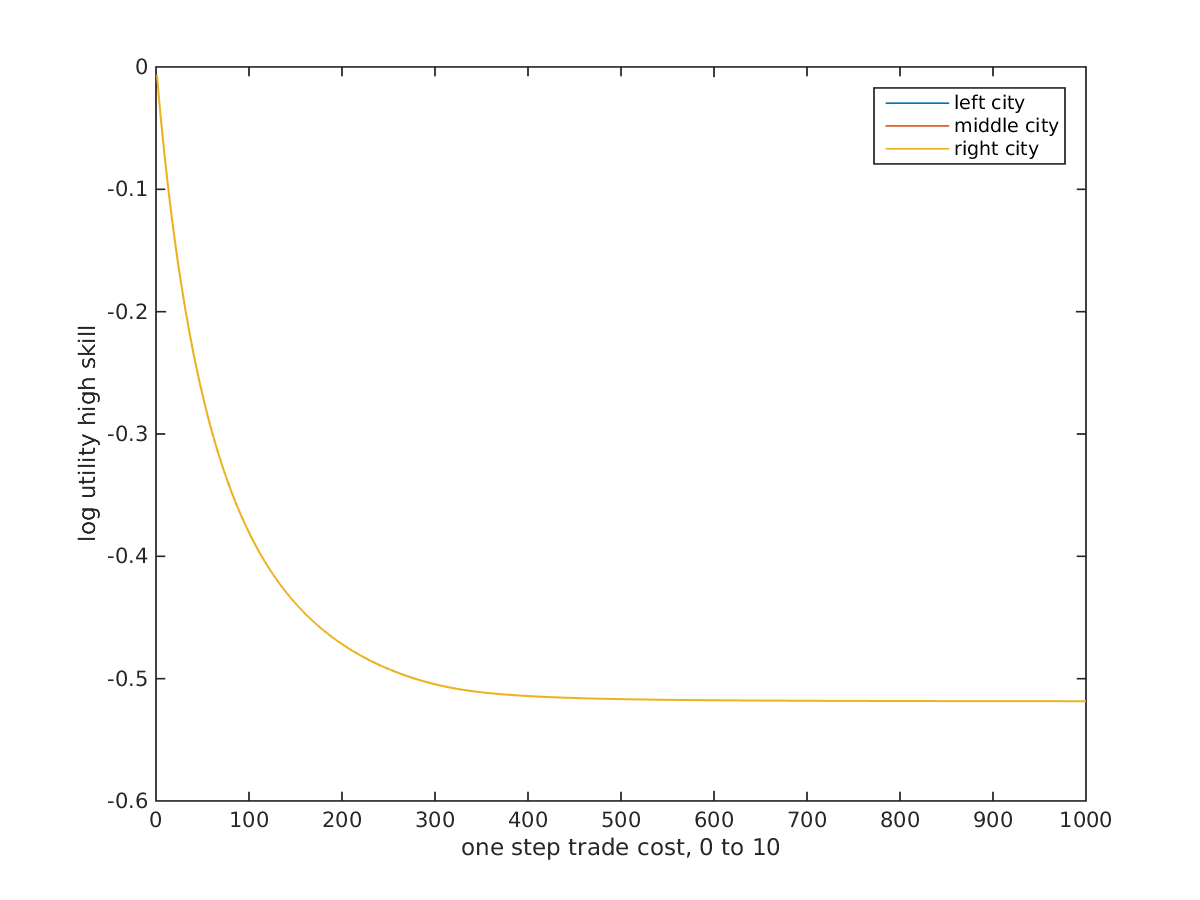
\includegraphics[width=.47\textwidth]{pics/tc/high_util.png}}
      \subfloat[Log low skill util]{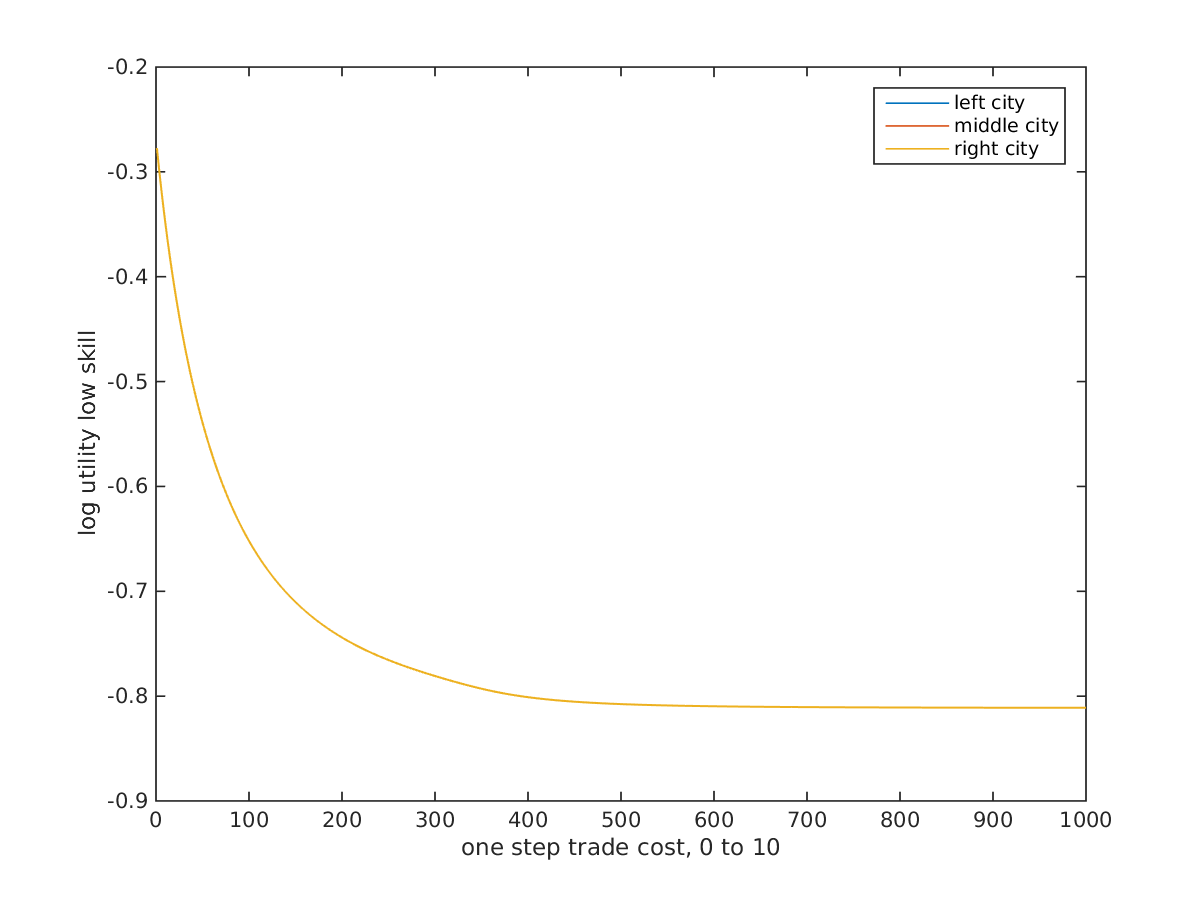
\includegraphics[width=.47\textwidth]{pics/tc/low_util.png}}
      \caption{Utilities fall as trade costs rise}
      \label{fig:tc_both_hurt}
    \end{figure}

    In the homothetic model, relative welfare is the same as the skill premium.  Figure \ref{tc_skill_prem} is the skill premium as we raise trade costs. The skill premium increases, which implies that low-skill workers are hurt more than high-skill workers by trade barriers.  The intuition is that by more or less shutting down trade, we move all high-skill workers into the same city.  Moving all high skill workers together mitigates the harm to them as they reap some benefit from additional aggomeration.  Low-skill workers get no such mitigation.  This result is the opposite of what one might expect from a comparative advantage story in which low trade barriers induce firms to outsource low-skill tasks.

    \begin{figure}[!ht]
      \centering
      {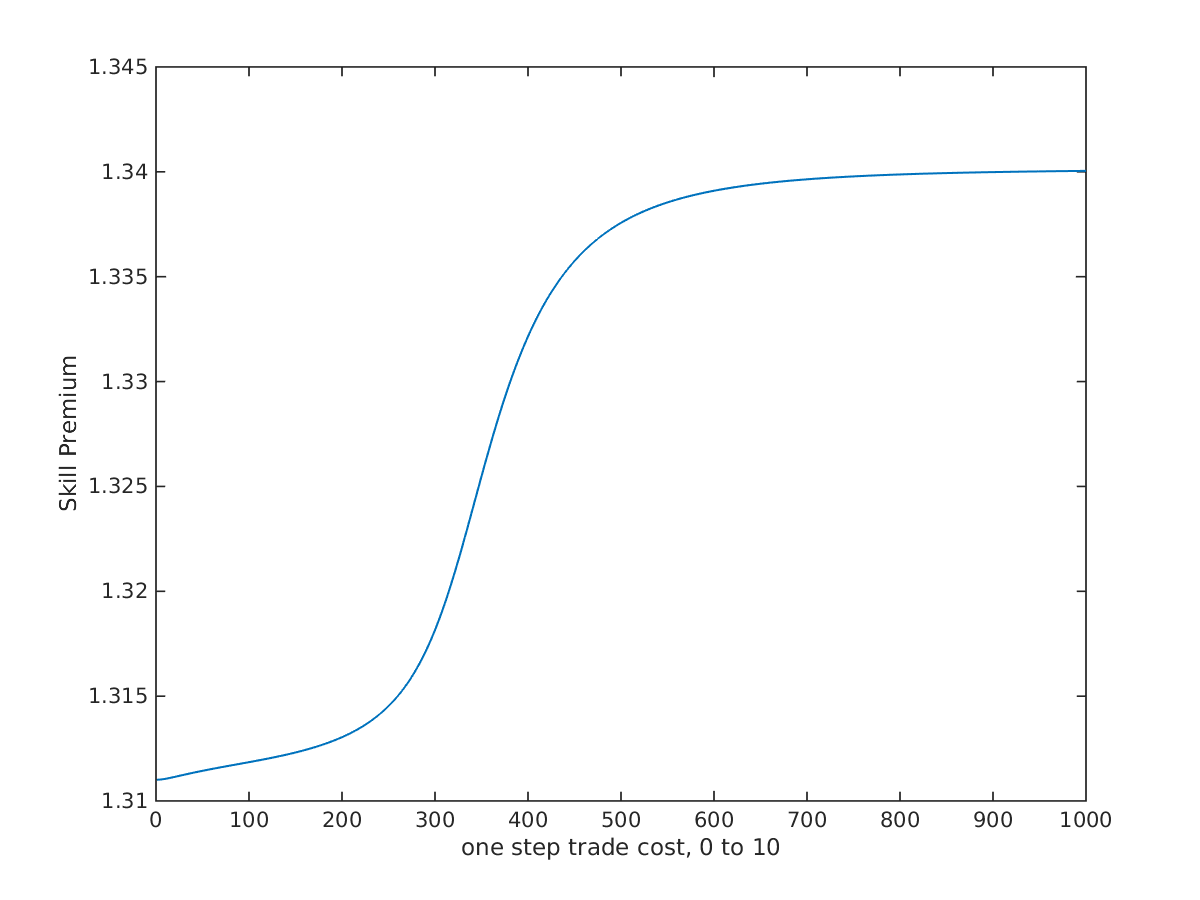
\includegraphics[width=2.5in]{pics/tc/skill_prem.png}}
      \caption{Skill premium as trade costs rise}
      \label{tc_skill_prem}
    \end{figure}

    In a second simulation exercise, we consider the type of parameters which generate two findings in the American data.  College share is higher in cities with higher population, and remote cities.  In order to generate these facts, we need to make the central city less attractive, as it benefits from the lowest trade costs of any city.  Because of its ease of trading, it the natural gathering point for high-skill agglomeration economies and a large population, which will give us the wrong correlations.  We can either increase the exogenous congestion $\bar{u}(i)$ in the central city, or we can increase the exogenous TFP $\bar{A}(i)$ in the edge cities.  In Figure \ref{fig:sim_col_share}, we raise the productivity levels in the edge cities from one, which is parity with the middle, to 1.5.  As expected, parity gives a higher college share and higher population in the center city. There is a flip in both population and college share as we raise exogenous TFP.

    \begin{figure}[!ht]
      \centering
      \subfloat[Total Population]{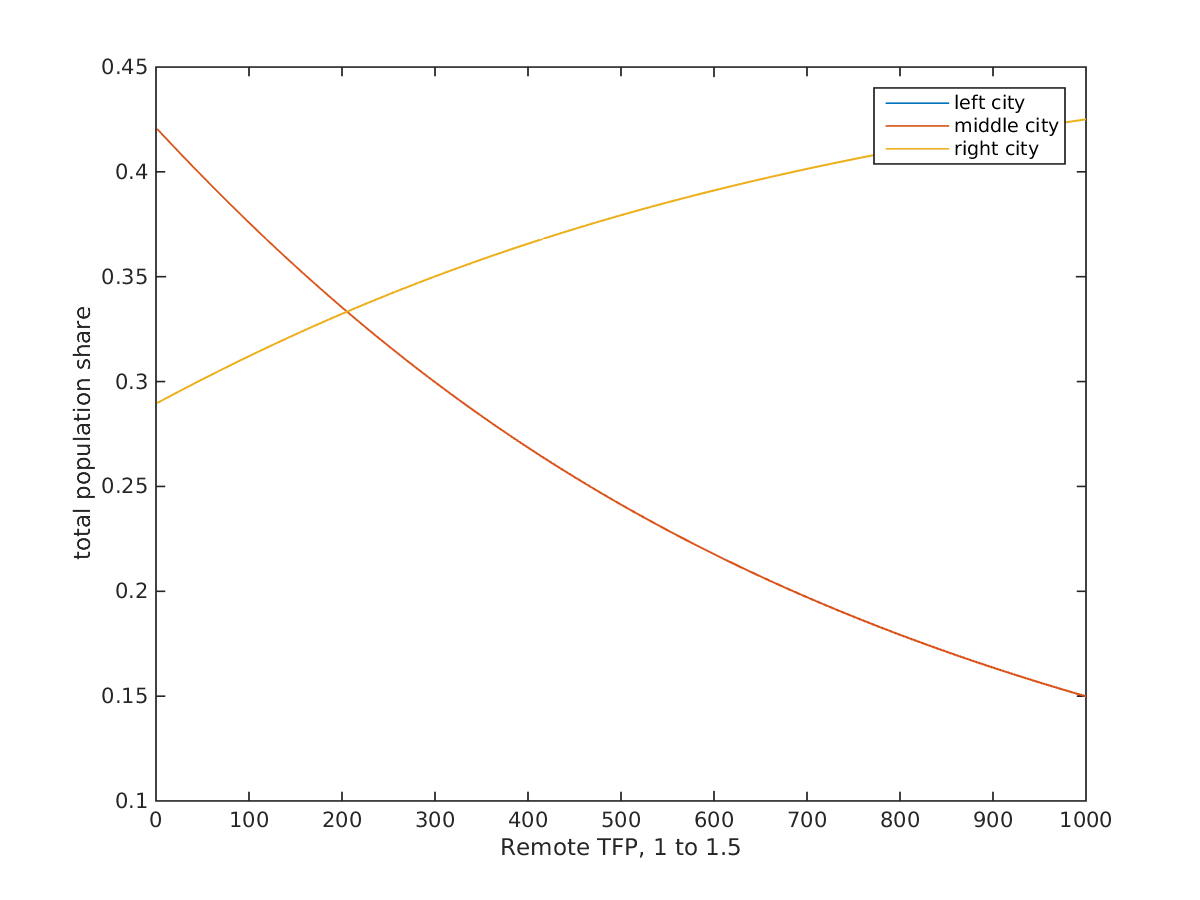
\includegraphics[width=.47\textwidth]{pics/tfp/pops.png}}
      \subfloat[College Share]{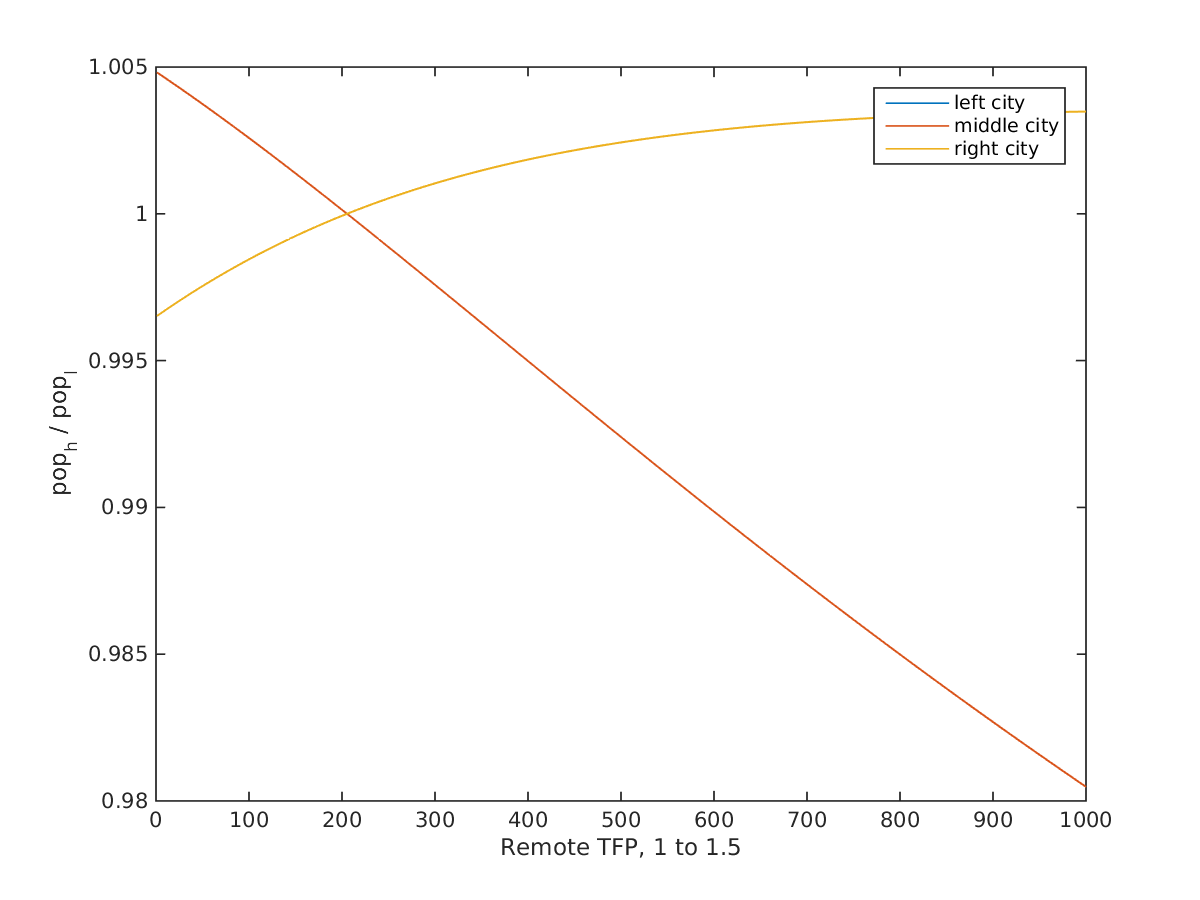
\includegraphics[width=.47\textwidth]{pics/tfp/pop_prem.png}}
      \caption{Population and College Share as TFP rises in remote locations}
      \label{fig:sim_col_share}
    \end{figure}

\section{Next steps}

While we have already found some compelling stylized facts, and written several empirical models, this project is still young, and in the near future we will be pushing forward on both the theoretical and empirical fronts.

We intend to combine the best features of the homothetic production structure with non-homothetic preferences.  This will allow us to examine skill premia varying over space as well as college shares.  We expect that the simulation of such a model will be more complicated.

We also plan on moving toward a full estimation of the model on real world geography as in \citet{allen2014trade}.  This will involve collecting data on internal trade between American locations, and implementing a fast marching algorithm to find the cheapest trade routes.  Once that is done, estimating the model should be relatively straight-forward.  A side benefit is that the internal trade measures will allow us to calculate a measure of remoteness even closer to that in the trade literature.

\section{Conclusion}

We have presented several new facts about the relationship between geography and inequality.  The skill premium correlates negatively with the remoteness of a city, and positively with its population.  The college share is positively correlated with both population and the remoteness of a city.

In order to understand the relationship between geography and inequality, we develop several models.  We learn that any model with homothetic preferences and free movement will deliver skill premia that are equalized everywhere.  We write down and solve a non-homothetic model which generates skill premia varying across space, but which has a stark production structure and is somewhat difficult to solve numerically.  We then write down a homothetic model which is richer and easier to work with.  

Finally we simulate the model and show that low-skill workers are hurt more than high-skill workers by trade barriers, and that we need remote locations to be innately attractive in order to generate the college share patterns we find in the data.

\newpage

\appendix

\section{Derivation of Non-Homothetic Equilibrium Conditions} 

According to $mcc_L$,
\begin{eqnarray}
	w_L(i) N_L(i) & = & \gamma_L \Big( w_H(i) N_H(i) + w_L(i) N_L(i) + p_z(i) (\bar{Z}-N(i)z_0) \Big) \nonumber
\end{eqnarray}
According to $mcc_z$, or equivalently by aggregating $X_z(i)$ in \eqref{eq:house_demand},
\begin{eqnarray}
	& & p_z(i)\bar{Z} = (1-\gamma_H-\gamma_L)Y(i) + (\gamma_H+\gamma_L)p_z(i)N(i)z_0 \nonumber \\
	& \Rightarrow &
    \label{eq:house_price}
	p_z(i) (\bar{Z}-N(i)z_0) = \frac{1-\gamma_H-\gamma_L}{\gamma_H+\gamma_L}(w_H(i) N_H(i) + w_L(i) N_L(i)) 
\end{eqnarray}
By using the implied equations from $mcc_L$ and $mcc_z$,
\begin{eqnarray}
	w_L(i) N_L(i)
	& = &  \gamma_L\Big(1+\frac{1-\gamma_H-\gamma_L}{\gamma_H+\gamma_L} \Big) \Big( w_H(i) N_H(i) + w_L(i) N_L(i) \Big) \nonumber \\
	& = &
	\Big(\frac{\gamma_L}{\gamma_H+\gamma_L} \Big) \Big( w_H(i) N_H(i) + w_L(i) N_L(i) \Big) \nonumber
\end{eqnarray}
Therefore,
\begin{equation}
	 w_L(i) N_L(i)= \frac{\gamma_L}{\gamma_H} w_H(i) N_H(i) \nonumber
\end{equation}
and,
\[
	 w_H(i) w_L(i) + w_L(i) N_L(i)= \frac{\gamma_H+\gamma_L}{\gamma_H} w_H(i) N_H(i) 
\]
Using \eqref{eq:house_price},
\[
	Y(i) = \frac{1}{\gamma_H} w_H(i)N_H(i) + p_z(i)N(i)z_0	
\]
By aggregating consumptions from \eqref{eq:house_demand},
\begin{eqnarray}
	X_H(s,i) & = & \Big[ \frac{p_H(s,i)}{P_H(i)} \Big]^{1-\sigma} \gamma_H \Big(Y(i)-p_z(i)N(i)z_0\Big) \nonumber \\
	X_L(s,i) & = & \gamma_L \Big(Y(i)-p_z(i)N(i)z_0\Big) \nonumber \\
	X_z(i) & = & (1-\gamma_H-\gamma_L)\Big(Y(i)-p_z(i)N(i)z_0\Big) + p_z(i)N(i)z_0 \nonumber
\end{eqnarray}
By replacing $Y(i)$,
\begin{eqnarray}
	X_H(s,i) & = & \Big[ \frac{p_H(s,i)}{P_H(i)} \Big]^{1-\sigma} w_H(i)N_H(i) \nonumber \\
	X_L(s,i) & = & \frac{\gamma_L}{\gamma_H} w_H(i)N_H(i) \nonumber \\
	X_z(i) & = & \frac{1-\gamma_H-\gamma_L}{\gamma_H}w_H(i)N_H(i) + p_z(i)N(i)z_0
\end{eqnarray}

According to $mcc_H$:
\begin{eqnarray}
    \label{eq:elim_wl}
	w_H(i) N_H(i) & = & \int_S \Big[ \frac{w_H(i) d(i,s)}{A_H(i) P_H(s)} \Big]^{1-\sigma} w_H(s) N_H(s) ~ds
\end{eqnarray}
Define
\begin{eqnarray}
    \label{eq:def_m}
	m(i)  & \equiv & \frac{P(i)}{P_H(i)} \nonumber \\ & = & 
	\gamma_{0}
	\Big( \frac{p_L(i)}{P_H(i)} \Big)^{\gamma_L}
	\Big( \frac{p_z(i)}{P_H(i)} \Big)^{1-\gamma_H-\gamma_L}
\end{eqnarray}
By welfare equalization, price index for $H$ in location $i$ can be written as
\begin{eqnarray}
	P_H(s) = \frac{w_H(s) -p_z(s)z_0}{z(s) W_H } \nonumber
\end{eqnarray}
We use \eqref{eq:house_price} to write $p_z(s)$ as a function of wages and labor supply: 
\[
	p_z(s) = \frac{1-\gamma_H -\gamma_L}{\gamma_H (\bar{Z}-N(s)z_0)}w_H(s)N_H(s)
\]
Note that holding other variables constant, $p_z(s)$ is higher if $w_H(s)$ is higher, if $N_H(s)$ is higher, if $N(s)$ is higher, or if $z_0$ is higher. Rewrite $P_H(s)$ as follows:
\begin{eqnarray}
	P_H(s) = \frac{w_H(s)g(s)}{m(s) W_H }	~,~where~~~
    \label{eq:def_g}
	g(s)=1- \frac{(1-\gamma_H -\gamma_L)N_H(s)z_0}{\gamma_H (\bar{Z}-N(s)z_0)} 
\end{eqnarray}
Combine \eqref{eq:elim_wl} and \eqref{eq:def_g},
\begin{eqnarray}
	& & N_H(i) w_H(i)^{\sigma}   = \nonumber \\
	& & \int_S W_H^{1-\sigma} m(s)^{1-\sigma} d(i,s)^{1-\sigma} A_H(i)^{\sigma-1} g(s)^{\sigma-1} N_H(s) w_H(s)^{\sigma}~ds  \nonumber
\end{eqnarray}
Combine \eqref{eq:nonhomo_price_index} and \eqref{def_g}, 
\begin{eqnarray}
    \label{eq:nonhomo_append_eq1}
	& & \Big[ \frac{w_H(i) c(i)}{m(i) W_H } \Big]^{1-\sigma} = \int_S w_H(s)^{1-\sigma}d(s,i)^{1-\sigma}A_H(s)^{\sigma-1}~ ds
\end{eqnarray}
which results in:
\begin{eqnarray}
    \label{eq:nonhomo_append_eq2}
 	w_H(i)^{1-\sigma} = \int_S W_H^{1-\sigma} m(i)^{1-\sigma} d(s,i)^{1-\sigma} A_H(s)^{\sigma-1} c(i)^{\sigma-1}  	w_H(s)^{1-\sigma}
 	~ ds
\end{eqnarray}
Define
\begin{eqnarray}
    \label{eq:def_B}
	B(i,s) = W_H^{1-\sigma} m(s)^{1-\sigma}  d(i,s)^{1-\sigma} A_H(i)^{\sigma-1} g(s)^{\sigma-1} \nonumber
\end{eqnarray}
Summarize the system of equations:
\begin{eqnarray}
    \label{eq:nonhomo_comp1}
	N_H(i) w_H(i)^{\sigma}  = \int_S B(i,s) N_H(s) w_H(s)^{\sigma}~ds \\
    \label{eq:nonhomo_comp2}
 	w_H(i)^{1-\sigma} = \int_S B(s,i) w_H(s)^{1-\sigma} ~ ds 
\end{eqnarray} 
Compare the pair \eqref{eq:nonhomo_append_eq1} and \eqref{eq:nonhomo_append_eq2} or its compact version \eqref{eq:nonhomo_comp1} and \eqref{eq:nonhomo_comp2} to the pair (8-9) in \citet{allen2014trade}. Two new components are $m(s)$ and $g(s)$ given by \eqref{eq:def_m} and \eqref{eq:def_g}. The new model nests that in \citet{allen2014trade}. If $\gamma_H=1,~\gamma_L=0$, then $m(s)\equiv 1$. If $z_0=0$, $g(s)\equiv 1$.  Compared with \citet{allen2014trade}, $B(s,i)$ is endogenous (because both $m(s)$ and $g(s)$ are endogenous). 

\section{Solving the homothetic model}

Rewrite \eqref{eq:def_b},
\begin{eqnarray}
	b(i) = \frac{1}{1 + \Big(\frac{\beta_L(i)}{\beta_H(i)}\Big)^{\varepsilon} \Big(\frac{w_L(i)}{w_H(i)}\Big)^{1-\varepsilon}} \nonumber
\end{eqnarray}
On the other hand, by definition,
\begin{eqnarray}
	b(i) = \frac{1}{1 + \frac{N_L(i)}{N_H(i)} \frac{w_L(i)}{w_H(i)}} \nonumber
\end{eqnarray}
Therefore,
\begin{eqnarray}
	\Big[\frac{\beta_L(i)}{\beta_H(i)}\Big]^{\varepsilon} \Big[\frac{w_L(i)}{w_H(i)}\Big]^{1-\varepsilon} = \frac{N_L(i)}{N_H(i)} \frac{w_L(i)}{w_H(i)} \nonumber \\
    \label{eq:homo_pop_share}
	\Big[\frac{\beta_L(i)}{\beta_H(i)}\Big]^{\varepsilon} \Big[\frac{w_L(i)}{w_H(i)}\Big]^{-\varepsilon}= \frac{N_L(i)}{N_H(i)} 
\end{eqnarray}
Under our specification of $\beta$'s, equation \eqref{eq:homo_pop_share} yields
\begin{eqnarray}
	\omega(i) \equiv \frac{w_H(i)}{w_L(i)} = \frac{\bar{\beta}_H}{\bar{\beta}_L} \frac{N_H(i)^{\tilde{\alpha}_H /\varepsilon}}{N_L(i)^{\tilde{\alpha}_L/\varepsilon}}
    \label{eq:homo_col_share}
\end{eqnarray}
where
\begin{eqnarray}
	\tilde{\alpha}_H & = & \varepsilon\alpha_H-1 \nonumber \\
	\tilde{\alpha}_L & = & \varepsilon\alpha_L-1 \nonumber
\end{eqnarray}
(note: interpret $\alpha_{\tau}$ as a force for skilled-bias technology or agglomeration for workers of type $\tau$; this force wins the standard force from demand if $\alpha_{\tau}>1/\varepsilon$.)

Since our demand system is homothetic, \textit{nominal} wage premium is the same as \textit{real} wage premium which in turn has to be constant across space by the notion of spatial equilibrium. In particular, \eqref{eq:homo_wel_eq} --welfare equalization across space-- implies:

\[
\omega(i) = \frac{W_H}{W_L} \equiv \omega.
\]

Using \eqref{eq:homo_col_share} we could express $N_L(i)$ as a function of $N_H(i)$ and $\omega$,
\begin{eqnarray}
    \label{eq:homo_N_L}
	N_L(i) = \Big[N_H(i)\Big]^{\tilde{\alpha}_H/\tilde{\alpha}_L} \Big[\frac{\bar{\beta}_H}{\bar{\beta}_L} \Big]^{\varepsilon/\tilde{\alpha}_L} \Big[\omega\Big]^{-\varepsilon/\tilde{\alpha}_L}
\end{eqnarray}
Total measure of low-skilled labor, 
$ \bar{N}_L = \int_S N_L(i)~di $, and 
 \eqref{eq:homo_N_L} pin down $\omega$ as a function of $N_H(i)$,
\begin{eqnarray}
    \label{eq:def_omega}
\omega = 
\Big[ \frac{\bar{\beta}_H}{\bar{\beta}_L}\Big]\Big[ \bar{N}_L
\Big]^{-\tilde{\alpha}_L/\varepsilon}
\Big[ \int_S N_H(i)^{\tilde{\alpha}_H/\tilde{\alpha}_L}~di \Big]^{\tilde{\alpha}_L/\varepsilon}
\end{eqnarray}

Further, note that income in $i$ equals
$\frac{1}{b(i)} w_H(i)N_H(i)$. We use equations \eqref{eq:homo_demand}
and \eqref{eq:homo_mcc},
\begin{eqnarray}
	w_H(i) N_H(i) b(i)^{-1} = 
	\int_S \Big[ \frac{c(i) d(i,s)}{A(i) P(s)} \Big]^{1-\sigma} w_H(s) N_H(s) b(s)^{-1} ~ds \nonumber
\end{eqnarray}
Equations \eqref{eq:homo_cost_min} and \eqref{eq:def_b} imply that 
\begin{eqnarray}
    \label{eq:def_tilde_c}
	c(i) & = & \tilde{c}(i) w_H(i) \nonumber \\
	where~~~ \tilde{c}(i) & = & 
	\Big[\beta_H(i)\Big] ^{\frac{\varepsilon}{1-\varepsilon}} \Big[b(i)\Big]^{\frac{-1}{1-\varepsilon}}
\end{eqnarray}

We replace for $c(i)$ from \eqref{eq:def_omega} and price index from \eqref{eq:homo_price_index} into \eqref{eq:homo_N_L}. After some algebra,
\begin{eqnarray}
    \label{eq:homo_eq_cond_append_1}
	& & w_H(i)^{\sigma} N_H(i) b(i)^{-1} \nonumber \\
	& & =  
	W_H^{1-\sigma} A(i)^{\sigma-1} \tilde{c}(i)^{1-\sigma}
	\int_S d(i,s)^{1-\sigma} u(s)^{\sigma-1} w_H(s)^{\sigma} N_H(s) b(s)^{-1}  ~ds \nonumber \\
\end{eqnarray}

On the other hand, equations \eqref{eq:homo_price_index} and \eqref{eq:homo_wel_eq} yield
\begin{eqnarray}
	\Big[ \frac{w_H(i) u(i)}{W_H } \Big]^{1-\sigma} = \int_S c(s)^{1-\sigma}d(s,i)^{1-\sigma}A(s)^{\sigma-1}~ ds \nonumber
\end{eqnarray}
which results
\begin{eqnarray}
    \label{eq:homo_eq_cond_append_2}
 	& & w_H(i)^{1-\sigma} = \nonumber \\ 
 	& & 
 	W_H^{1-\sigma} u(i)^{\sigma-1} 
 	\int_S  d(s,i)^{1-\sigma} A(s)^{\sigma-1}  \tilde{c}(s)^{1-\sigma} w_H(s)^{1-\sigma}
 	~ ds 
\end{eqnarray}

Equations \eqref{eq:homo_eq_cond_append_1} and \eqref{eq:homo_eq_cond_append_2} give us two systems of integral equations. By the following relation, we can reduce the two systems into one: 
\begin{eqnarray}
    \label{eq:homo_eq_cond_append_3}
	\frac{w_H(i)^{\sigma}N_H(i)A(i)^{1-\sigma}\tilde{c}(i)^{\sigma-1}}{b(i)} = \phi w_H(i)^{1-\sigma} u(i)^{1-\sigma}
\end{eqnarray}
where $\phi > 0$ is a constant. As long as \eqref{eq:homo_eq_cond_append_3} holds, then system \eqref{eq:homo_eq_cond_append_1} holds if and only if system \eqref{eq:homo_eq_cond_append_2} holds. So, along with \eqref{eq:homo_eq_cond_append_3}, it is enough to solve either only \eqref{eq:homo_eq_cond_append_1} or only \eqref{eq:homo_eq_cond_append_2}.

\section{Homothetic solution algorithm}

We can simulate the homothetic model with the following steps:

\begin{enumerate}
\item Guess $N_H(i)$ for all $i$.
\item Calculate $\omega$ according to \eqref{eq:def_omega}. Then plug it in \eqref{eq:homo_N_L} to calculate $N_L(i)$.
\item Calculate $b(i)
= 1/(1 + \frac{N_L(i)}{N_H(i)} \frac{1}{\omega}) $
\item Calculate $\tilde{c}(i)$ according to \eqref{eq:def_tilde_c}.
\item Calculate $w_H(i)$ according to \eqref{eq:homo_eq_cond_append_3} (up to a scale imposed by $\phi$)
\item Let $f(i)=w_H(i)^{1-\sigma}$, $\kappa=W_H^{1-\sigma}$, and
\[
K(s,i) = u(i)^{\sigma-1} d(s,i)^{1-\sigma} A(s)^{\sigma-1} \tilde{c}(s)^{1-\sigma}
\]
Then, rewrite \eqref{eq:homo_eq_cond_append_2} as follows:
\[
f(i) = \kappa \int_S K(s,i) f(s)~ds
\]
Get updated, scaled version of $f_u(i)$ using \eqref{eq:homo_eq_cond_append_2}: 
\begin{eqnarray}
    f^u(i) = \frac{\int_S K(s,i) f(s)~ds}{\int_S \int_S K(s,i) f^u(s)~ds di}\nonumber
\end{eqnarray}
\item Use $f^u$ to calculate updated scaled $N^u_H(i)$ using \eqref{eq:homo_eq_cond_append_3}. 
\item Finaly, correctly scale the updated $N^u_H(i)$.  Find $\phi$ such that $\bar{N}_h=\int_S N^u_H(i)~di$.
\item If $N^u_H(i) = N_H(i)$, stop.  Otherwise, use updated $N^u_H(i)$ as new guess in step (1). 
\end{enumerate}

\newpage

\bibliographystyle{apa.bst}
\bibliography{/home/veryshuai/Documents/bib/biglist.bib}

\end{document}
